\documentclass[11pt,a4paper]{article}
\usepackage[utf8]{inputenc}
\usepackage{amsmath}
\usepackage{amsfonts}
\usepackage{amssymb}
\usepackage{enumerate}
\usepackage{graphicx}


\title{Lab 01\\Arquitectura de Computadores \\ Sección 2}
\author{Joaquín Ramírez}
\begin{document}
\maketitle
\begin{enumerate}
\item Dados dos números de 4-bits, se comparan los pares i-ésimos, $i = 0, 1, 2, 3$ con XOR gates. Finalmente se conectan en un AND gate, el cual solo se activará cuando todos los pares estén activados.
\begin{figure}[h!]
\centering
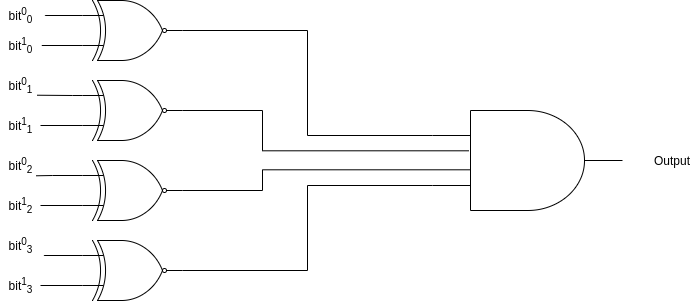
\includegraphics[scale=0.4]{1.png} 
\end{figure}
\item Se adjunta un archivo .asc con la simulación del ejercicio anterior.
\item Los diagramas con logic gates de las funciones booleanas son los \\siguientes:
\begin{itemize}
\item NOT: se divide un input en dos y pasa por un NAND, lo que significa que simplemente se invertirán los posibles casos 0 y 1.
\begin{figure}[h!]
\centering
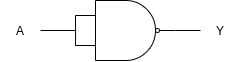
\includegraphics[scale=0.5]{2.png} 
\end{figure}
\item AND: se niega un NAND con el NOT del ejercicio anterior.
\begin{figure}[h!]
\centering
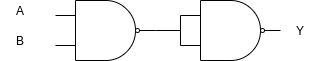
\includegraphics[scale=0.5]{3.png} 
\end{figure}
\\
\item OR: ya que la tabla de verdad del NAND es la misma que la del OR pero con los inputs invertidos, se niegan los inputs y se aplica un NAND después.
\begin{figure}[h]
\centering
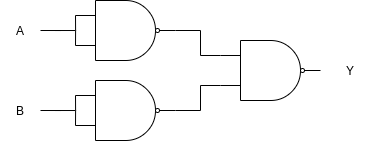
\includegraphics[scale=0.5]{4.png} 
\end{figure}
\item NOR: al negar el OR, sacando dos inputs de su resultado, se obtiene el NOR.
\begin{figure}[h!]
\centering
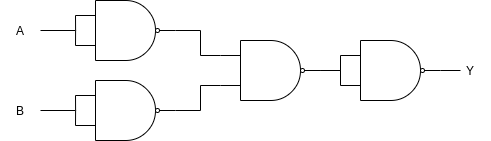
\includegraphics[scale=0.5]{5.png} 
\end{figure}
\item XOR: el diagrama con menos compuertas es el siguiente.
\begin{figure}[h!]
\centering
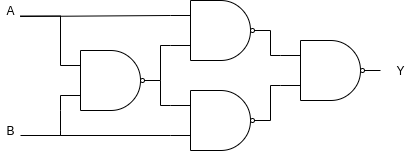
\includegraphics[scale=0.5]{6.png} 
\end{figure}
\\Sin embargo, una opción más sencilla de obtener es con el Teorema de De Morgan y la Suma de Productos. De esta manera:\\ $Y = \overline{A}B + \overline{B}A = \overline{(\overline{\overline{A}}+\overline{B})(\overline{A}+\overline{\overline{B}})} = \overline{(\overline{B}+A)(\overline{A}+B)}$
\begin{figure}[h!]
\centering
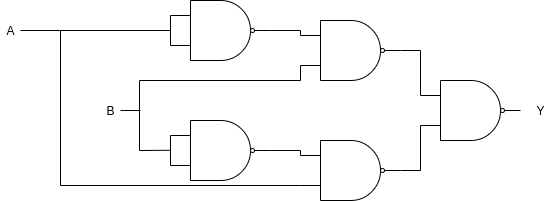
\includegraphics[scale=0.45]{7.png} 
\end{figure}

\end{itemize}
\end{enumerate}
\end{document}